\section{Проектирование программного средства}
\label{sec:design}

Проектирование – процесс определения архитектуры, компонентов, интерфейсов и других характеристик системы или её части. Результатом проектирования является проект – целостная совокупность моделей, свойств или характеристик, описанных в форме, пригодной для последующей реализации системы. Оно, наряду с анализом требований, является частью большой стадии жизненного цикла системы, называемой определением системы. 

Проектирование системы направлено на представление системы, соответствующее предусмотренной цели, принципам и замыслам; оно включает оценку и принятие решений по выбору таких компонентов системы, которые отвечают её архитектуре и укладываются в предписанные ограничения.

\subsection{Описание используемых паттернов проектирования}
\label{sec:modeling:patterns}

Шаблон проектирования или паттерн в разработке программного обеспечения — повторяемая архитектурная конструкция, представляющая собой решение проблемы проектирования в рамках некоторого часто возникающего контекста.

Обычно шаблон не является законченным образцом, который может быть прямо преобразован в код; это лишь пример решения задачи, который можно использовать в различных ситуациях. Объектно-ориентированные шаблоны показывают отношения и взаимодействия между классами или объектами, без определения того, какие конечные классы или объекты приложения будут использоваться.

<<Низкоуровневые>> шаблоны, учитывающие специфику конкретного языка программирования, называются идиомами. Это хорошие решения проектирования, характерные для конкретного языка или программной платформы, и потому не универсальные.

На наивысшем уровне существуют архитектурные шаблоны, они охватывают собой архитектуру всей программной системы. Алгоритмы по своей сути также являются шаблонами, но не проектирования, а вычисления, так как решают вычислительные задачи. В сравнении с полностью самостоятельным проектированием, шаблоны обладают рядом преимуществ. Основная польза от использования шаблонов состоит в снижении сложности разработки за счёт готовых абстракций для решения целого класса проблем. 

Шаблон даёт решению своё имя, что облегчает коммуникацию между разработчиками, позволяя ссылаться на известные шаблоны. Таким образом, за счёт шаблонов производится унификация деталей решений: модулей, элементов проекта, — снижается количество ошибок. Применение шаблонов концептуально сродни использованию готовых библиотек кода.

Правильно сформулированный шаблон проектирования позволяет, отыскав удачное решение, пользоваться им снова и снова. Набор шаблонов помогает разработчику выбрать возможный, наиболее подходящий вариант проектирования. 

Хотя легкое изменение кода под известный шаблон может упростить понимание кода, по мнению Стива Макконнелла, с применением шаблонов могут быть связаны две сложности. Во-первых, слепое следование некоторому выбранному шаблону может привести к усложнению программы. Во-вторых, у разработчика может возникнуть желание попробовать некоторый шаблон в деле без особых оснований. 

\subsubsection{}Одиночка
\

В данном программном средстве используется паттерн <<Одиночка>>.
Одиночка (англ. Singleton) — порождающий шаблон проектирования, гарантирующий, что в однопроцессном приложении будет единственный экземпляр некоторого класса, и предоставляющий глобальную точку доступа к этому экземпляру~\cite{design_patterns}. У класса есть только один экземпляр, и он предоставляет к нему глобальную точку доступа. 

\begin{figure}[ht]
\centering
    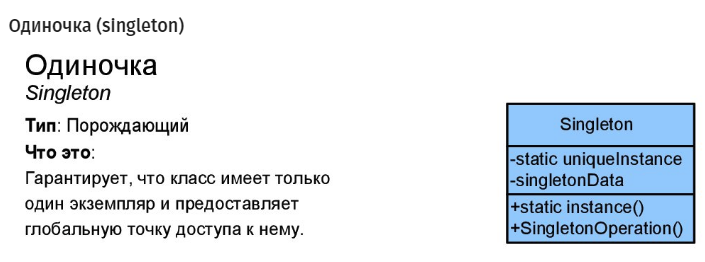
\includegraphics[scale=0.6]{design_singleton_pattern.png}
    \caption{Паттерн проектирования <<Одиночка>>}
    \label{sec:modeling:singleton}
\end{figure}

Существенно то, что можно пользоваться именно экземпляром класса, так как при этом во многих случаях становится доступной более широкая функциональность. Например, к описанным компонентам класса можно обращаться через интерфейс, если такая возможность поддерживается языком.

Глобальный <<одинокий>> объект — именно объект, а не набор процедур, не привязанных ни к какому объекту — бывает нужен:

\begin{itemize}
    \item если используется существующая объектно-ориентированная библиотека;
    \item если есть шансы, что один объект когда-нибудь превратится в несколько;
    \item если интерфейс объекта (например, игрового мира) слишком сложен и не стоит засорять основное пространство имён большим количеством функций;
    \item если, в зависимости от каких-нибудь условий и настроек, создаётся один из нескольких объектов. Например, в зависимости от того, ведётся лог или нет, создаётся или настоящий объект, пишущий в файл, или <<заглушка>>, ничего не делающая.
\end{itemize}

Минусы:
\begin{itemize}
    \item если объект нужен уже при инициализации, он может быть затребован раньше, чем будет создан;
    \item бывает, что объект нужен не всегда. В таком случае его создание можно пропустить.
\end{itemize}

\subsubsection{}Фабрика
\

Factory -- это паттерн создания объектов (creational pattern)~\cite{design_patterns}. Данный шаблон проектирования предоставляет интерфейс для создания экземпляров некоторого класса. В момент создания наследники могут определить, какой класс инстанциировать.

\begin{figure}[ht]
\centering
    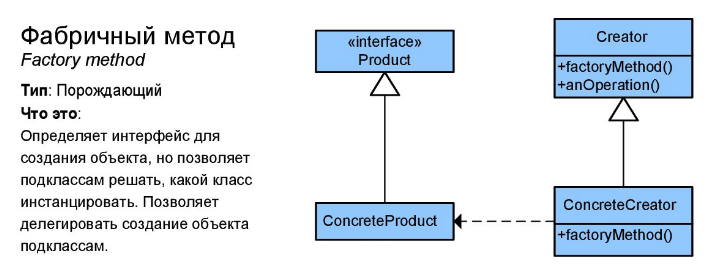
\includegraphics[scale=0.6]{design_factory_pattern.png}
    \caption{Паттерн проектирования <<Фабрика>>}
    \label{sec:modeling:factory}
\end{figure}

Иными словами, Фабрика делегирует создание объектов наследникам родительского класса. Это позволяет использовать в коде программы не специфические классы, а манипулировать абстрактными объектами на более высоком уровне.
\subsection{Проектирование алгоритма работы программы}
\label{sec:design:algorithm}

На рисунке~\ref{sec:design:main_algorithm_scheme} представлена схема алгоритма работы программного средства создания веб-приложений с помощью готовых графических компонентов. 
На ней отражены такие возможные действия, доступные для выполнения, как применение пресетов и компонентов, редактирование свойств компонентов, удаление компонентов. 

\begin{figure}[ht]
\centering
    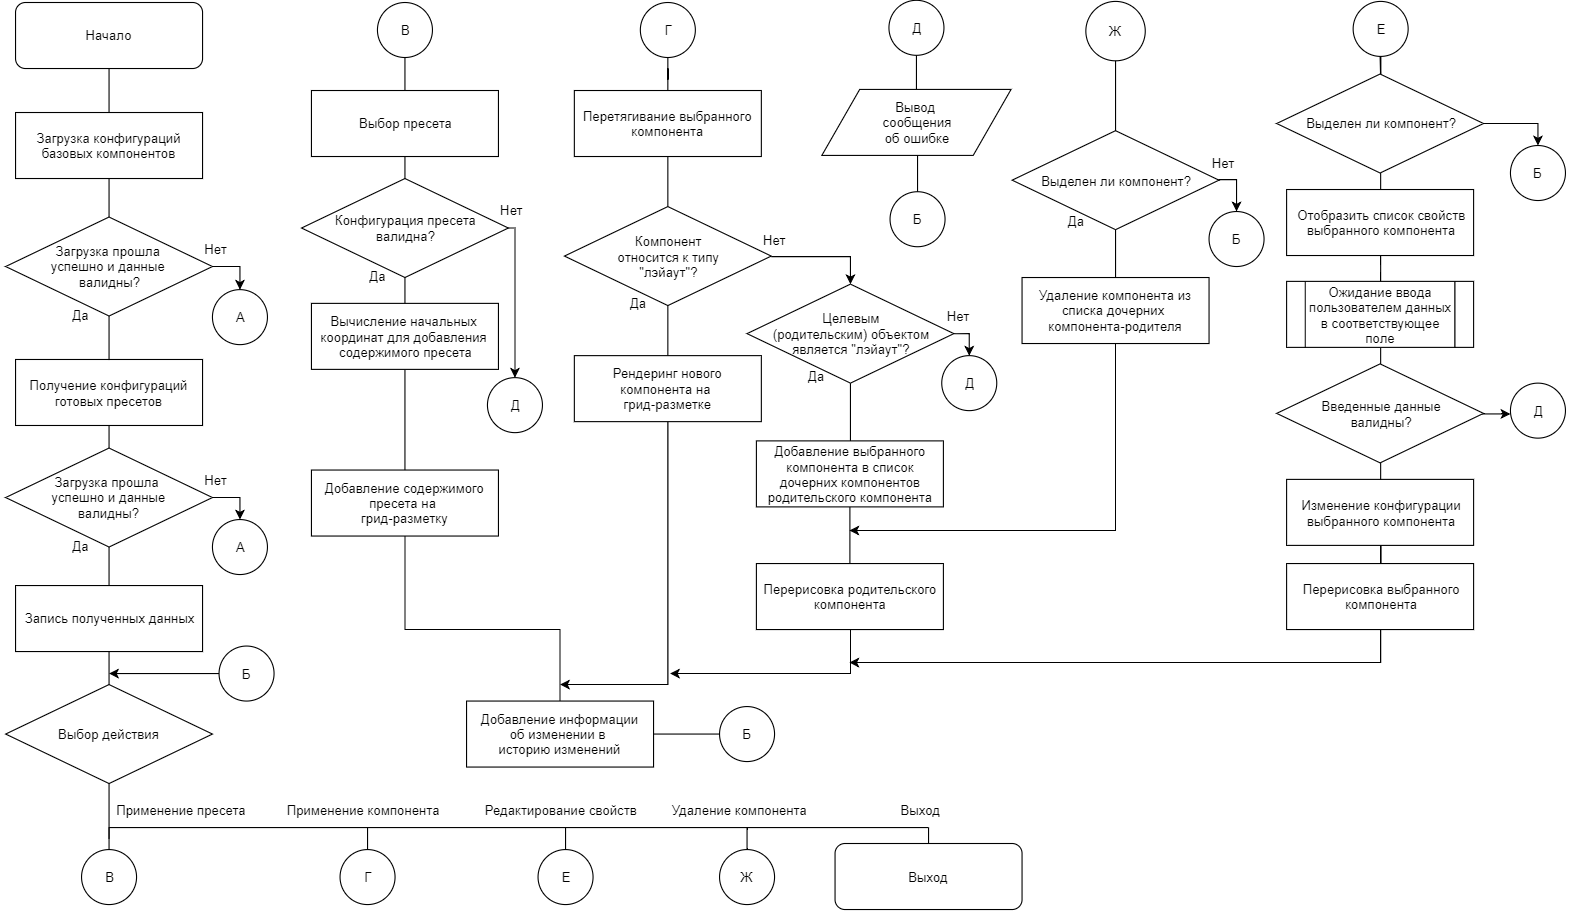
\includegraphics[scale=0.40]{Main_algorithm_scheme.png}
    \caption{Диаграмма прецедентов приложения}
    \label{sec:design:main_algorithm_scheme}
\end{figure}
    
В зависимости от конкретного действия, каждое содержит в себе собственные шаги реализации. 
Так при выборе действия <<Применение компонента>> происходит отрисовка одного компонента, перетянутого пользователем на грид-разметку, а при выборе <<Применение пресета>> происходит отрисовка целой совокупности компонентов. <<Редактирование свойств>> содержит в себе проверку введённых данных на корректность и процесс измненения свойств выбранного компонента. <<Удаление компонента>> осуществляется при выбора компонента и нажатии кнопки удаления, в таком случае все дочерние элементы (если они есть) также удаляются, после чего родительский компонент (если выбранный удаляемый компонент не был помещен непосредственно на грид-разметку) также перерисовывается. Каждое действие влечет за собой дополнительное действие в виде запоминания выполненных действий в истории изменений, чтобы в случае необходимости <<откатить>> произошедшие изменения.

\subsection{Диаграмма последовательности программного средства}
\label{sec:modeling:sequence}

Диаграмма последовательности (Sequence Diagram) – диаграмма, на которой показаны взаимодействия объектов, упорядоченные по времени их проявления.

Основными элементами диаграммы последовательности являются обозначения объектов (прямоугольники), вертикальные линии, отображающие течение времени при деятельности объекта,и стрелки, показывающие выполнение действий объектами. На данной диаграмме объекты располагаются слева направо. Ее недостатком является то, что она занимает много места.

Диаграммы последовательности, описывающие сценарии Business Use Case в виде последовательности обмена сообщениями между объектами - действующими лицами и объектами-исполнителями. Такие диаграммы помогают явно определить в модели обязанности каждого исполнителя в виде набора операций класса.

На диаграмме последовательности изображаются только те объекты, которые непосредственно участвуют во взаимодействии. Ключевым моментом для диаграмм последовательности является динамика взаимодействия объектов во времени.

В UML диаграмма последовательности имеет как бы два измерения. Первое слева направо в виде вертикальных линий, каждая из которых изображает линию жизни отдельного объекта, участвующего во взаимодействии. Крайним слева на диаграмме изображается объект, который является инициатором взаимодействия. Правее изображается другой объект, который непосредственно взаимодействует с первым. Таким образом, все объекты на диаграмме последовательности образуют некоторый порядок, определяемый очередностью или степенью активности объектов при взаимодействии друг с другом.

\begin{figure}[ht]
\centering
    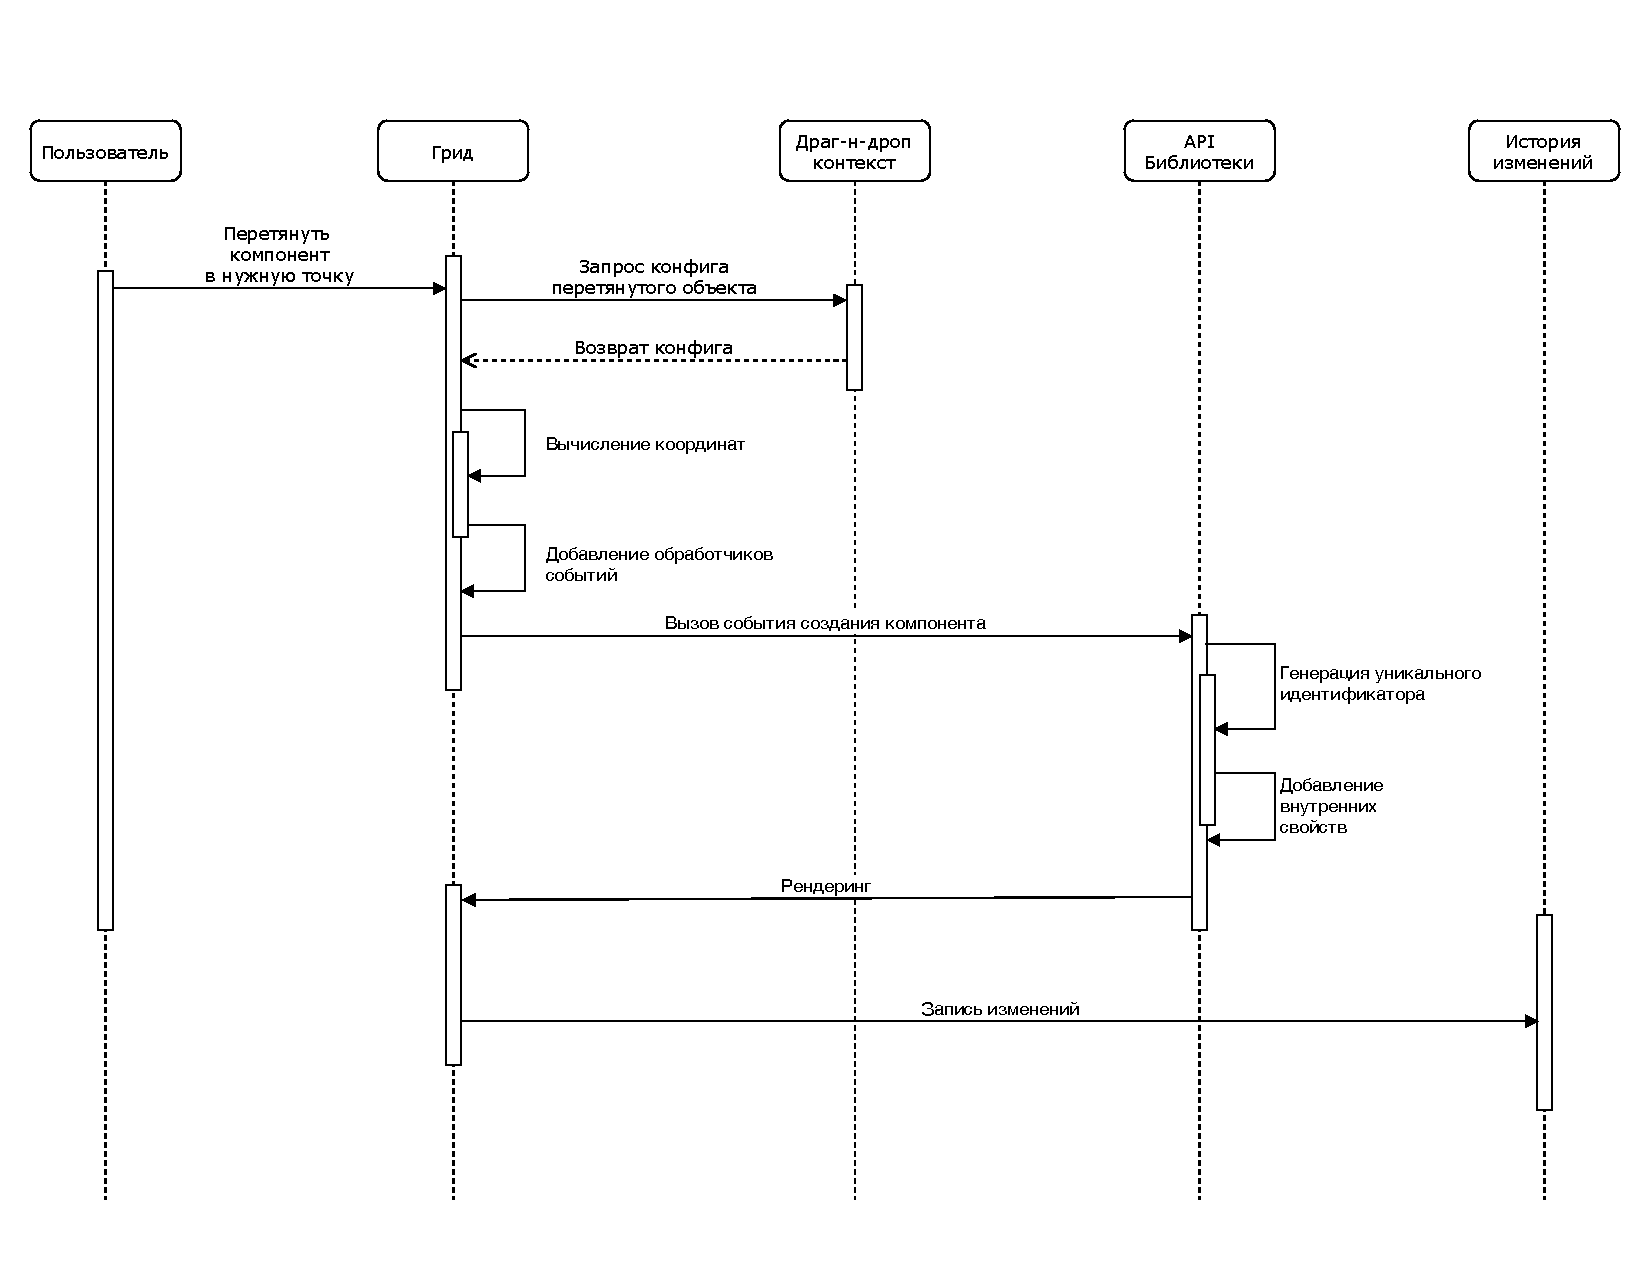
\includegraphics[scale=0.59]{schema_sequence.pdf}
    \caption{Диаграмма последовательности использования предопределенных конфигураций графических компонентов}
    \label{sec:design:sequence_diagram}
\end{figure}

На рисунке~\ref{sec:design:sequence_diagram} представлена диаграмма последовательности применения предопределенных конфигураций графических компонентов программного средства создания веб-приложений с помощью готовых графических компонентов. 
На ней отражен процесс, происходящий в программе каждый раз при перетягивании пользователем компонента на грид.\pagebreak

